\documentclass[letterpaper]{article}
\usepackage[margin=1in]{geometry}
\usepackage{amsmath}
\usepackage{listings,color,enumitem}
\usepackage{graphicx}
\usepackage{float}

%\linespread{1.15}

\title{Homework \#3: SLAM using EKF}
\author{ Matthew Swenson }
\date{\today}

\begin{document}
  \maketitle
\thanks{Shivang Baveja and Abdul Zafar were instrumental in my completion of this assignment.}
    \newpage

\section{2D LInear SLAM}
\subsection*{A}
\begin{align}
    & h_o = r_t - r_{t-1} & h_m = l_t - r_t & 
\end{align}
\begin{align}
    & H_o = r_t - r_{t-1} & H_m = l_t - r_t & 
\end{align}




\subsection*{C}
$$
l = \left(\begin{array}{c} x+\cos\left(\mathrm{\beta}+n_{\beta }+\mathrm{\theta}\right)\,\left(n_{r}+r\right)\\ y+\sin\left(\mathrm{\beta}+n_{\beta }+\mathrm{\theta}\right)\,\left(n_{r}+r\right) \end{array}\right) 
$$
\subsection*{D}
$$
\left(\begin{array}{c} r_{\mathrm{est}}\\ \beta _{\mathrm{est}} \end{array}\right)
=
\left(\begin{array}{c} \sqrt{{\left(l_{x}-x\right)}^2+{\left(l_{y}-y\right)}^2}\\ -\theta+\text{atan2}\left(l_{y}-y,l_{x}-x\right) \end{array}\right)
$$
\subsection*{E}
Defining $\delta_x = l_x - x$, $\delta_y = l_y - y$, and $q = \delta_x^2 + \delta_y^2$


and using the identities $\frac{\partial}{\partial x}atan2(y,x) = -\frac{y}{x^2+y^2}$ and $\frac{\partial}{\partial y}atan2(y,x) = -\frac{x}{x^2+y^2}$ 

we can write 

$$
H_p = \left(\begin{array}{ccc} -\frac{\delta _{x}}{\sqrt{q}} & -\frac{\delta _{y}}{\sqrt{q}} & 0\\ \frac{\delta _{y}}{q} & -\frac{\delta _{x}}{q} & -1 \end{array}\right)
$$

\subsection*{F}
Using the same identities: 
$$
H_l =\left(\begin{array}{cc} \frac{\delta _{x}}{\sqrt{q}} & \frac{\delta _{y}}{\sqrt{q}}\\ -\frac{\delta _{y}}{q} & \frac{\delta _{x}}{q} \end{array}\right) 
$$
We don't calculate other covariances because our initial assumption is that the landmarks are independent, or at least
that we can't tell which landmarks are dependent.
\section*{2}
\subsection*{A}
There are six landmarks.
\subsection*{B}
\begin{figure}[H]
    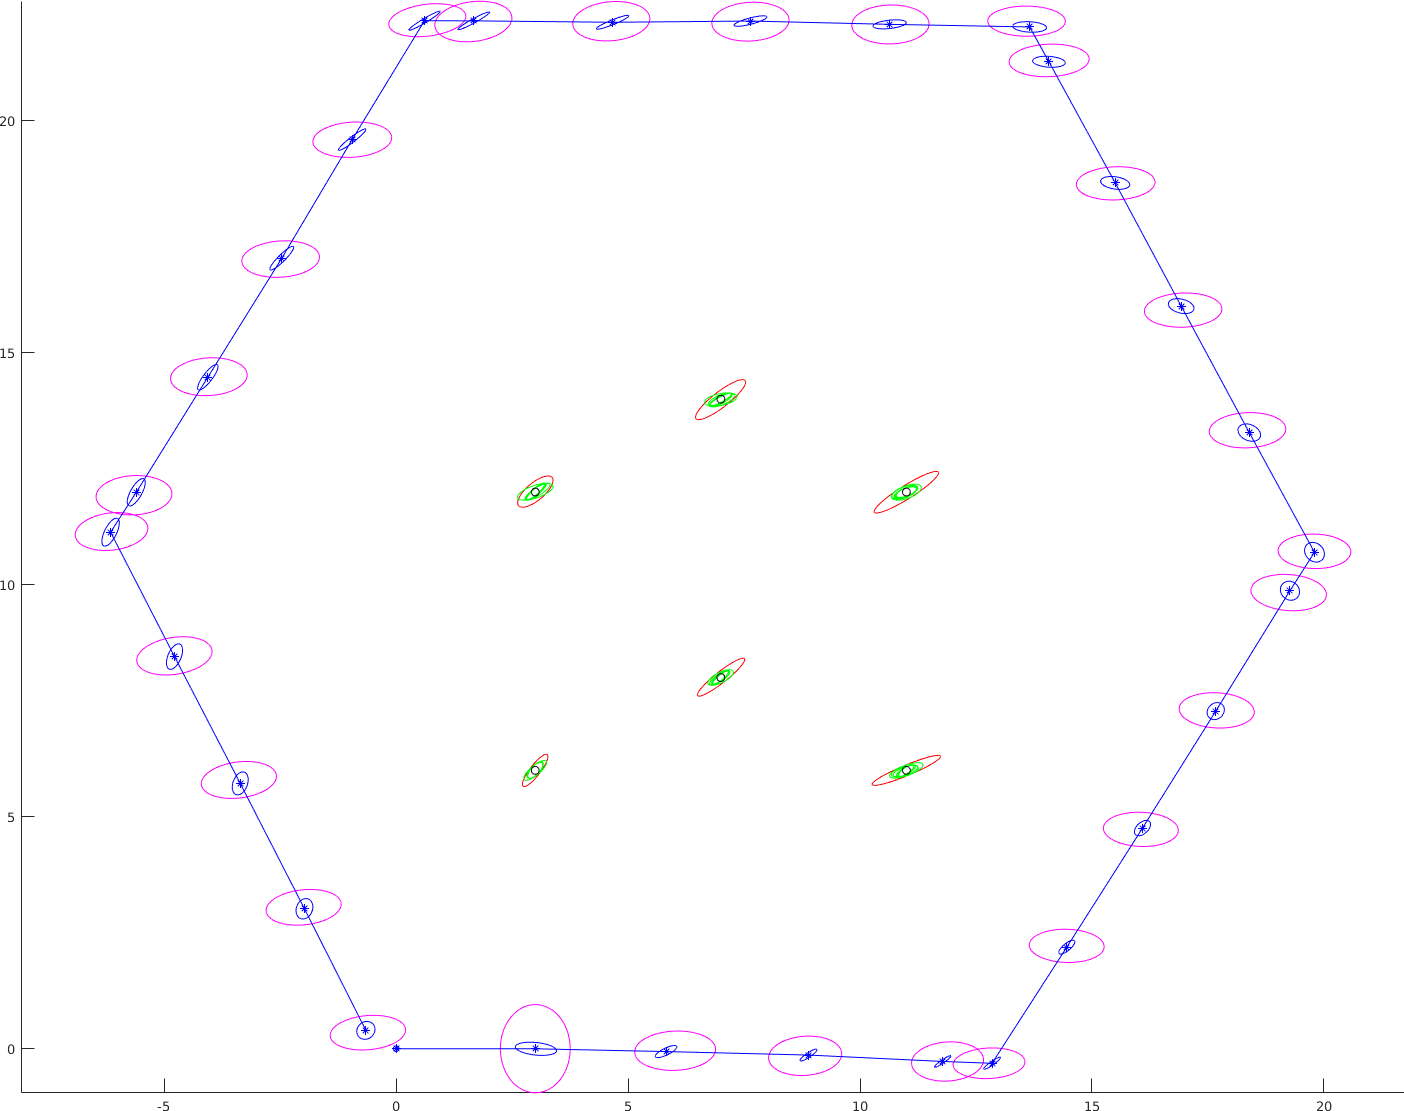
\includegraphics[width=\textwidth]{EKF_slam/standard_result.png}
    \caption{The results of the EKF algorithm with standard weights.}
\end{figure}
\subsection*{C}
EKF-SLAM allows recursive estimation of map features and robot position. The more accurately the 
robot is localized, the more accurately the landmarks can be localized, and the more accurately the landmarks 
are localized the more accurately the robot can be localized. This reinforcing relationship is evidenced by the 
decreasing size of the ovals as the robot moves around its path.
\subsection*{D}
Each of the landmark ground truths is inside its estimation ellipse, which means the algorithm is correctly locating 
the landmarks. 

For each landmark 1 through 6 I calculated the following distances:
\begin{table}[H]
\centering
\begin{tabular}{|l|l|l|l|l|l|l|}
\hline
\textbf{Landmark}    & 1          & 2          & 3         & 4          & 5          & 6          \\ \hline
\textbf{Euclidean}   & 0.002166   & 0.0048962  & 0.0057513 & 0.0050097  & 0.0016491  & 0.0063981  \\ \hline
\textbf{Mahalanobis} & 8.0392e-05 & 0.00033551 & 0.0004054 & 0.00039031 & 2.8445e-05 & 0.00046589 \\ \hline
\end{tabular}
\end{table}

I interpret to mean that not only are the average estimates very close to the ground truths, these estimates are significant 
and trustworthy because they have low variance.

\section*{3}
\subsection*{A}
Roughly speaking, the covariance matrix fills up because the landmarks are dependent. We also assume the landmarks
and the robot state are independent, which is not necessarily correct. 

\subsection*{B}
\begin{figure}[H]
    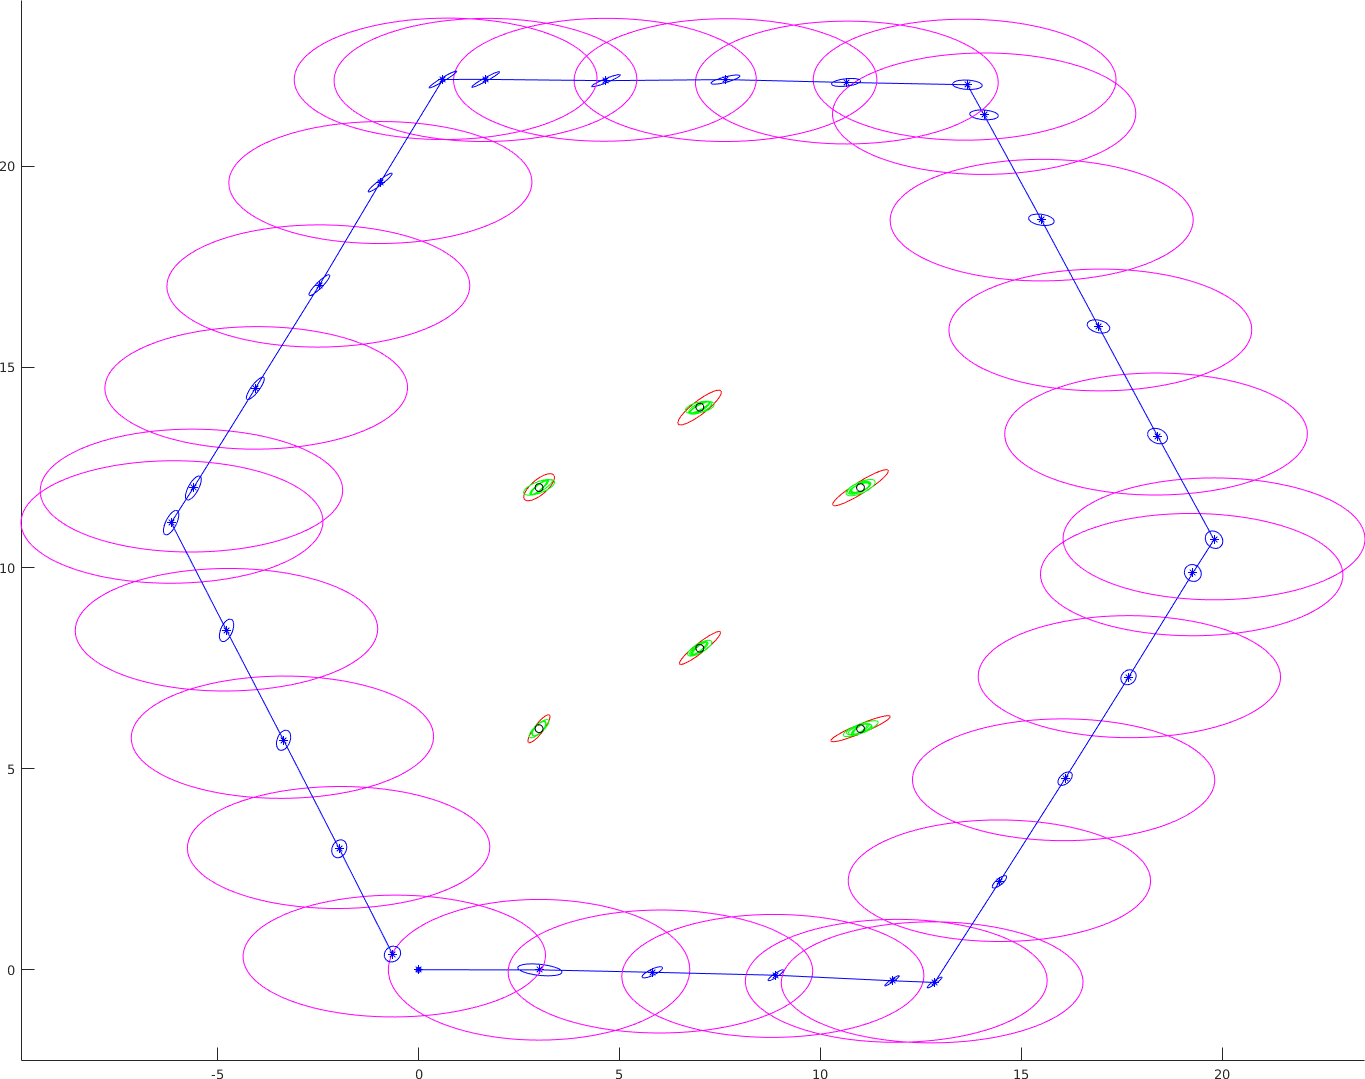
\includegraphics[width=\textwidth]{EKF_slam/5xworsecontrol.png}
    \caption{The results of the EKF algorithm with 5x uncertainty in control values. Note that the estimation of the robot position becomes much less accurate but the landmark estimation is roughly the same.}

\end{figure}
\begin{figure}[H]
    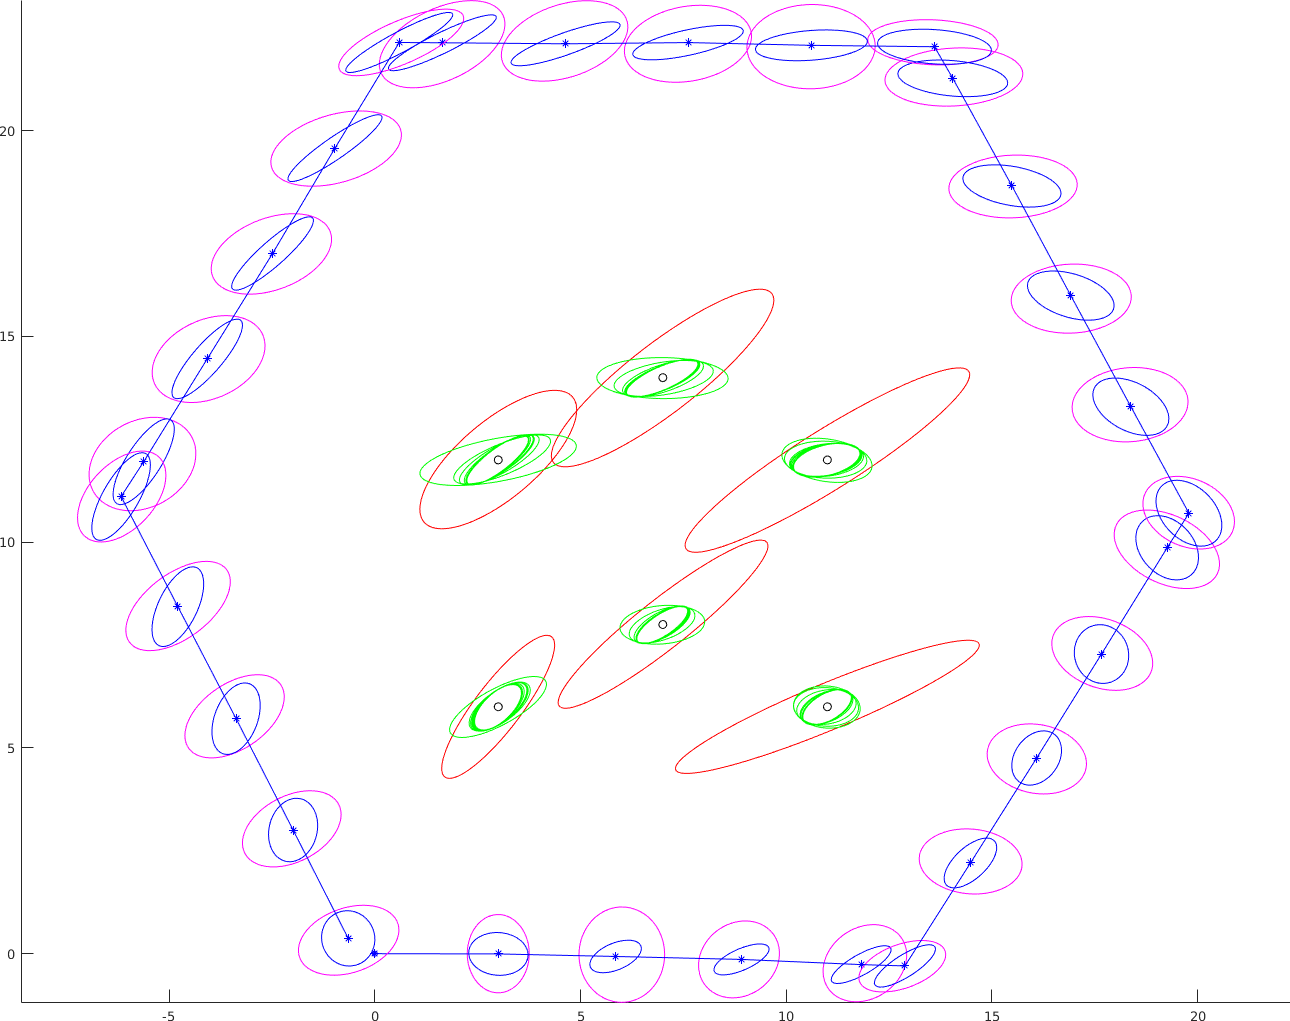
\includegraphics[width=\textwidth]{EKF_slam/5xworsemeasurement.png}
    \caption{The results of the EKF algorithm with 5x uncertainty in measurement values. Note that both the landmark estimaiton and the pose estimation get worse.}

\end{figure}

\end{document}

